\documentclass[a4paper]{article}

\usepackage[english]{babel}
\usepackage[utf8]{inputenc}
\usepackage{amsmath}
\usepackage{hyperref}
\usepackage[multiple]{footmisc}
\usepackage{graphicx}
\usepackage{algorithm}
\usepackage{algpseudocode}
\usepackage{pifont}
\usepackage{subfigure}
\usepackage[colorinlistoftodos]{todonotes}
\usepackage{tikz}
\usepackage{neuralnetwork}


\title{{Predicting rainfall using Ensembles of Ensembles.\footnote{The online competition is available at the Kaggle website \href{https://inclass.kaggle.com/c/how-s-the-weather}{\url{https://inclass.kaggle.com/c/how-s-the-weather}}. The name of the team was \texttt{foo\_bar}}
}\footnote{This work was does as a part of the project for  \href{http://sli.ics.uci.edu/Classes/2015W-273a}{CS 273: Machine Learning, Fall 2014}, taught by \href{http://www.ics.uci.edu/~ihler/}{Prof. Alexander Ihler}.}}
\author{{Prolok Sundaresan, Varad Meru, and Prateek Jain}\footnote{Prolok Sundaresan: Student\# 66008474, Varad Meru: Student\# 26648958, Prateek Jain: Student\# 28321844}\\
  University of California, Irvine\\
  \texttt{\{sunderap,vmeru,prateekj\}@uci.edu}}
\date{}

\begin{document}
\maketitle

\begin{abstract}
Regression is an approach for modeling the relationship between data \texttt{X} and the dependent variable \texttt{y}. In this report, we present our experiments with multiple approaches, ranging from Ensemble of learners to Deep Learning Networks on the weather modeling data to predict the rainfall. The competition was held on the online data science competition portal `Kaggle'. The results for weighted ensemble of learners gave us a top-10 ranking, with the testing root-mean-squared-error being 0.5587.
\end{abstract}

\section{Introduction}
The fundamental task of the in-class Kaggle competition is to predict the amount of rainfall at a particular location using satellite data.


\section{The DataSet}
\label{sec:dataset}

\subsection{Features}

\subsection{Visualizing the Data}
Visualizing the data was a difficult task since the data was in 91 dimensions.
In order to look for patterns in the data and visualized it, we applied SVD technique to reduce the dimensionality of the features to 2 principle dimensions. Then we applied k means clustering with k=5 on the data with 91 dimensions and plotted the assignments in the 2 dimensional transformed feature space. We saw patterns in the data(show the figure). Espeically some points were densely clustered and some were sparse.

To visualize it better, we transformed the feature in 3 dimensional space, and saw that the points were clustered around 3 planes.

\begin{figure}
\centering
\subfigure[Visualizing the data in 3 dimensions]{
    \label{fig:nn-runs}
    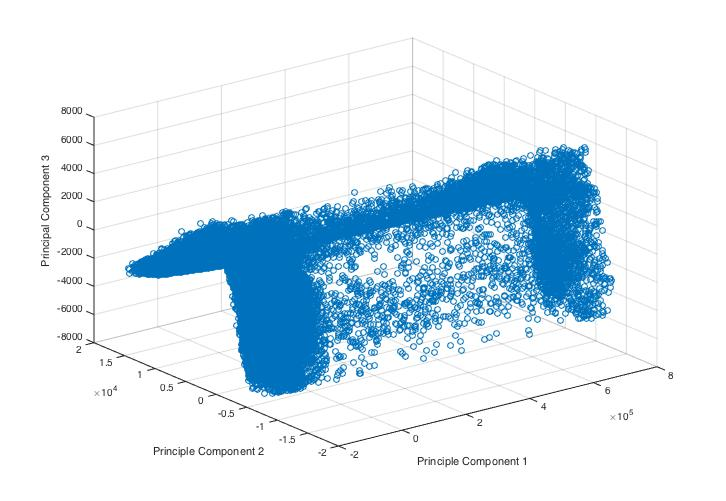
\includegraphics[scale=0.5]{3DViz}
}
\subfigure[Train-Validation-Test error plot for 20 neuron hidden layer]{
    \label{fig:nn-runs20}
    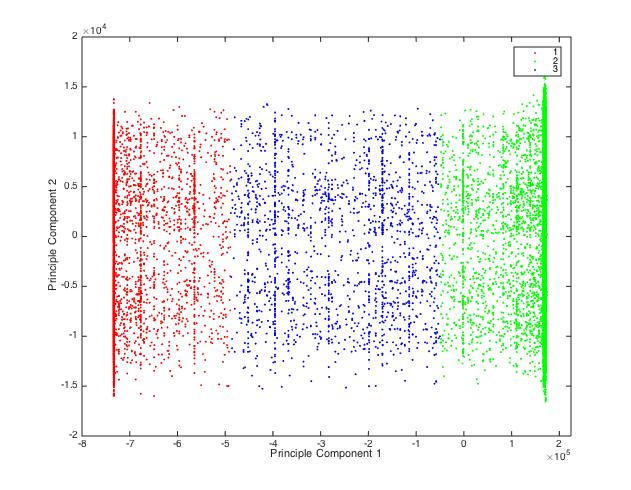
\includegraphics[scale=0.5]{pc2D}
}
\caption[]{Visualizing the principle components of Data}
\label{fig:nn-runs}
\end{figure}
 
\section{Machine Learning Models}
\label{sec:models}
\subsection{Mixture of Experts}
As seen from our visualization, we could identify two highly dense areas of the feature data on either side of a region of sparsely distributed data. The idea behind using the mixture of experts approach was, that intuitively, it would be difficult for a single regressor to fit the dataset, since the distribution is non-uniform.

We decided to split the data into clusters. To cluster the data, we used several intitialization of the k means algorithm with the kmeans++ intitialization. We decided to use K=3 for 3 evident clustering of the data in the visualization.

Since each of the clusters got a subset of a points from the original dataset, number of data points per cluster was not a very large number. Our concern with this was that any model we chose would overfit the data in its cluster. 

Therefore, we used the ensemble method of gradient boosting for each of the clusters. Since, in gradient boosting, we start with an underfitting model and then gradually add complexity, the chances of overfitting would be less in this model. We decided to use Decision stumps as our regressors for the boosting algorithm.

\begin{figure}[h]
\centering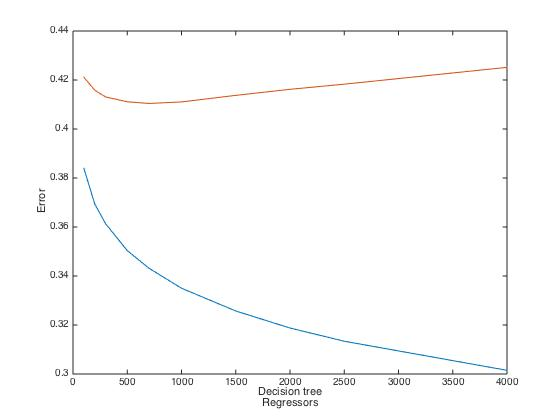
\includegraphics[width=1\linewidth,height=7cm]{mixtureOfExperts}
\caption{Mixture of Experts Error}
\end{figure}

\subsection{Neural Networks}
We implemented various types of neural networks, ranging from single layer networks to 3-layer sigmoidal neural networks.
\subsubsection*{Single Layer Network}

\begin{figure}[h]
\centering
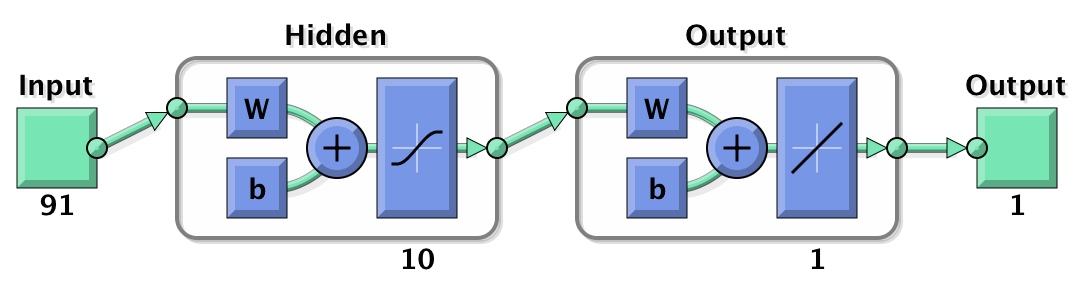
\includegraphics[scale=0.50]{nnarch.png}
\caption{Single Layer Architecture.}
\end{figure}

We build the neural network using the MATLAB's Neural-Network-Toolkit and PyBrain library implemented in Python. For the MATLAB implementation, there were various runs made for different number of neurons in the hidden layer. The architecture of the neural network can be seen \autoref{fig:nnarch}. The \autoref{fig:nn-runs} show the train-test-validation plots for different network architectures. The dataset was distributed into 70\% (Training), 20\% (Validation) and 10\% (Testing) section for the neural network to run. The \autoref{tab:nn_errors} shows the performance of the models learned. It was seen that the neural networks started to overfit as the number of neurons were increased more than 40.%

\begin{table}[h]
\centering
\begin{tabular}{ | l | l | l |}
\hline
\# of Neurons & Training Error (RMSE) & Testing Error (RMSE) \\ \hline
10 & 0.5986 & 0.61341 \\ \hline
20 & 0.5875 & 0.61301 \\ \hline
50 & 0.5852 & 0.62889 \\ \hline
\end{tabular}
\label{tab:nn_errors}
\caption{RMSE Error rates for different network architectures.}
\end{table}

It was observed that the learner could not learn very accurately as the data a lot as the data was not much for the neural network to learn on.

\begin{figure}
\centering
\subfigure[Train-Validation-Test error plot for 10 neuron hidden layer]{
    \label{fig:nn-runs}
    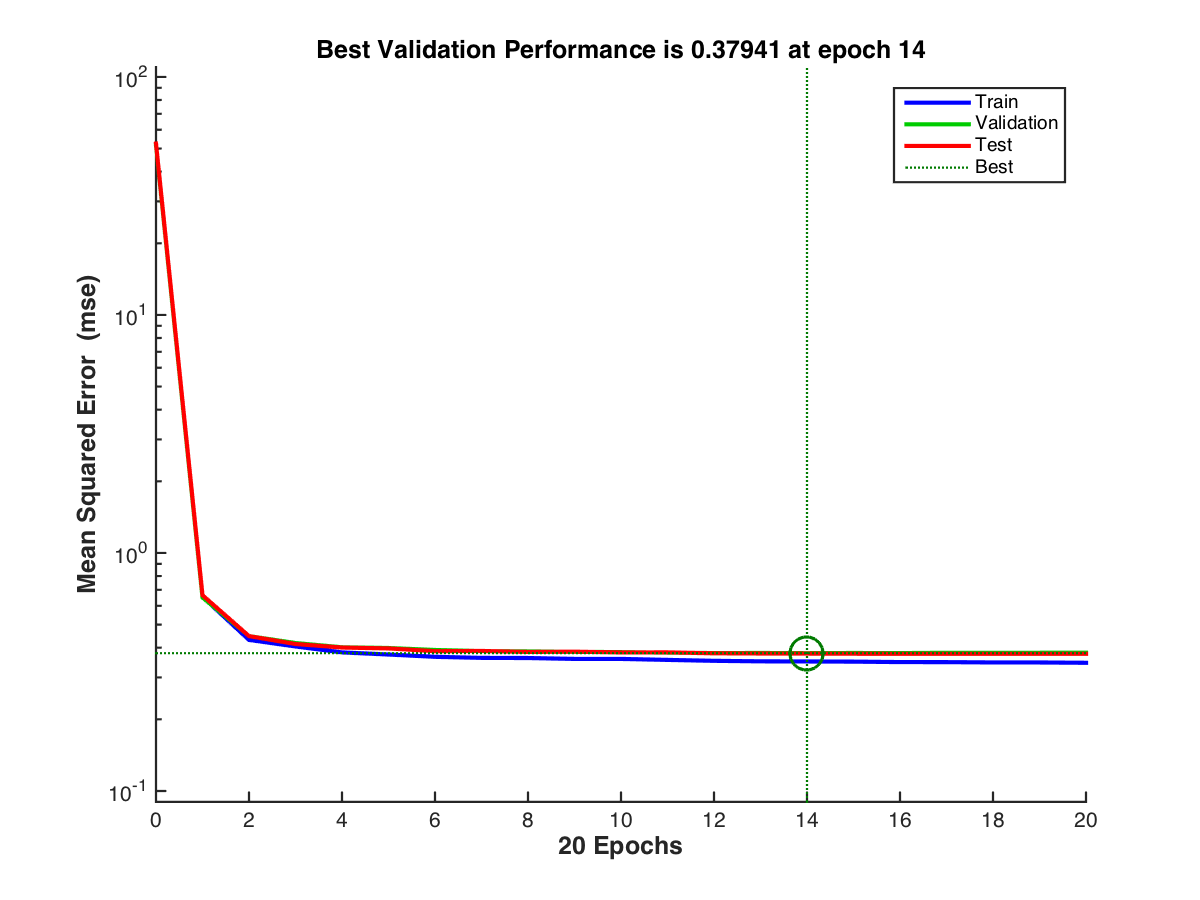
\includegraphics[scale=0.28]{plotperform.png}
}
\subfigure[Error distribution histogram for 10 neuron hidden layer]{
    \label{fig:nn-runs}
    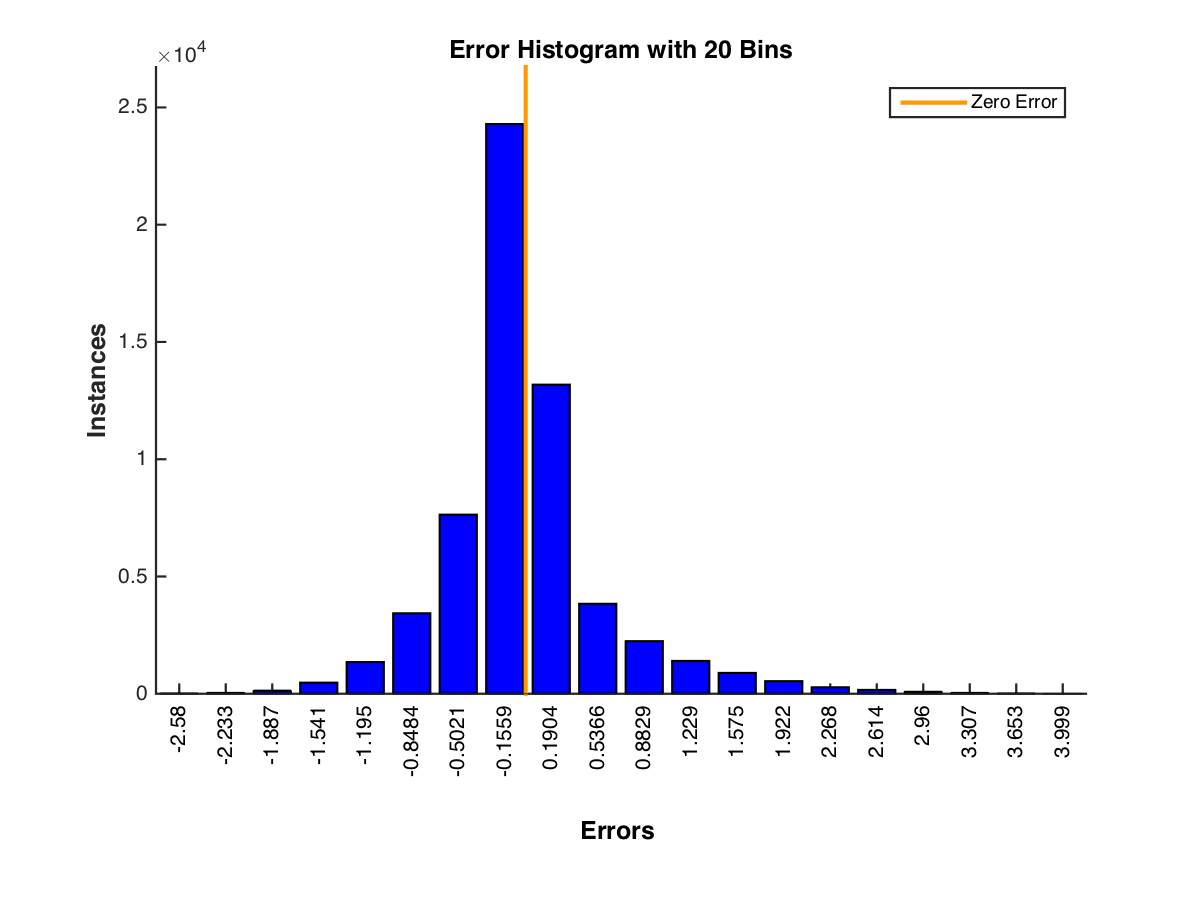
\includegraphics[scale=0.28]{ploterrhist.png}
}
\subfigure[Train-Validation-Test error plot for 20 neuron hidden layer]{
    \label{fig:nn-runs20}
    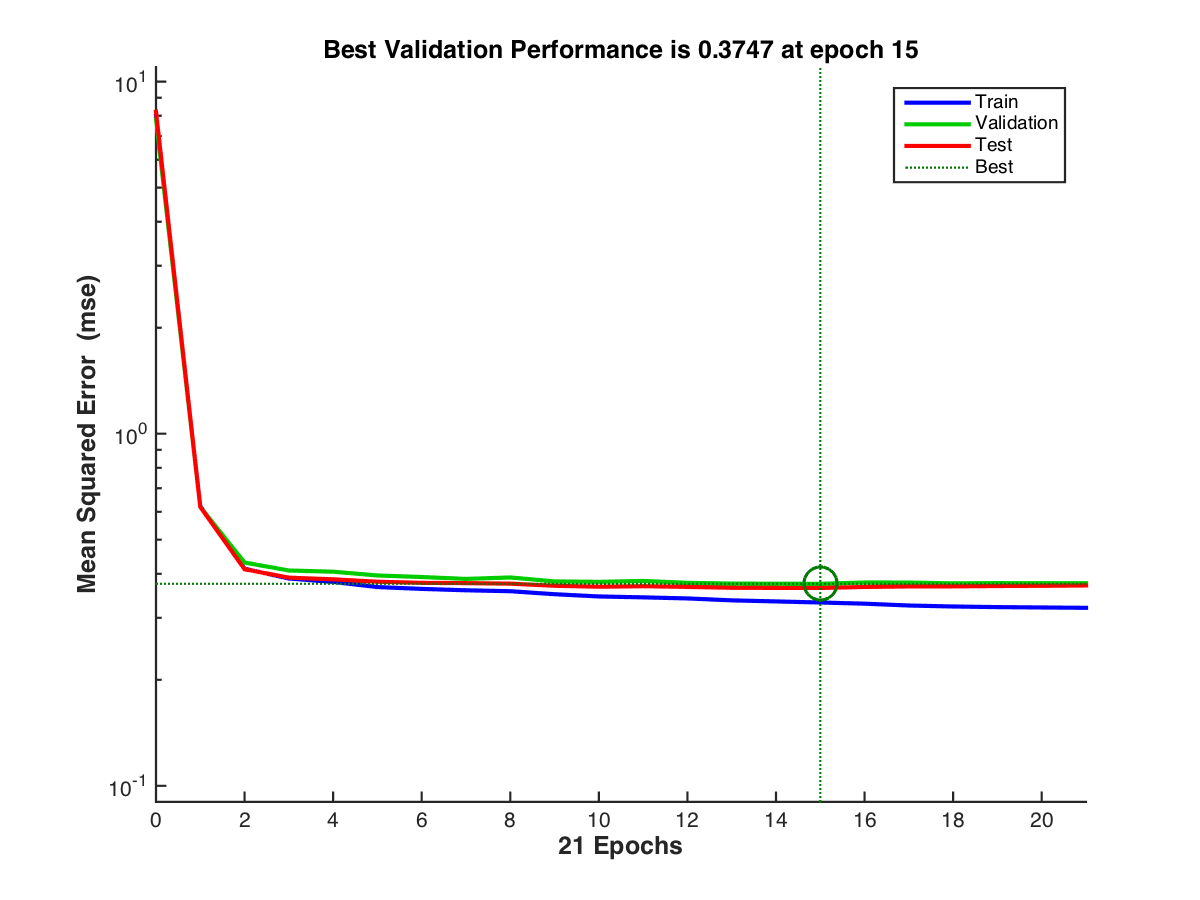
\includegraphics[scale=0.28]{plotperform_20.png}
}
\subfigure[Error distribution histogram for 20 neuron hidden layer]{
    \label{fig:nn-runs}
    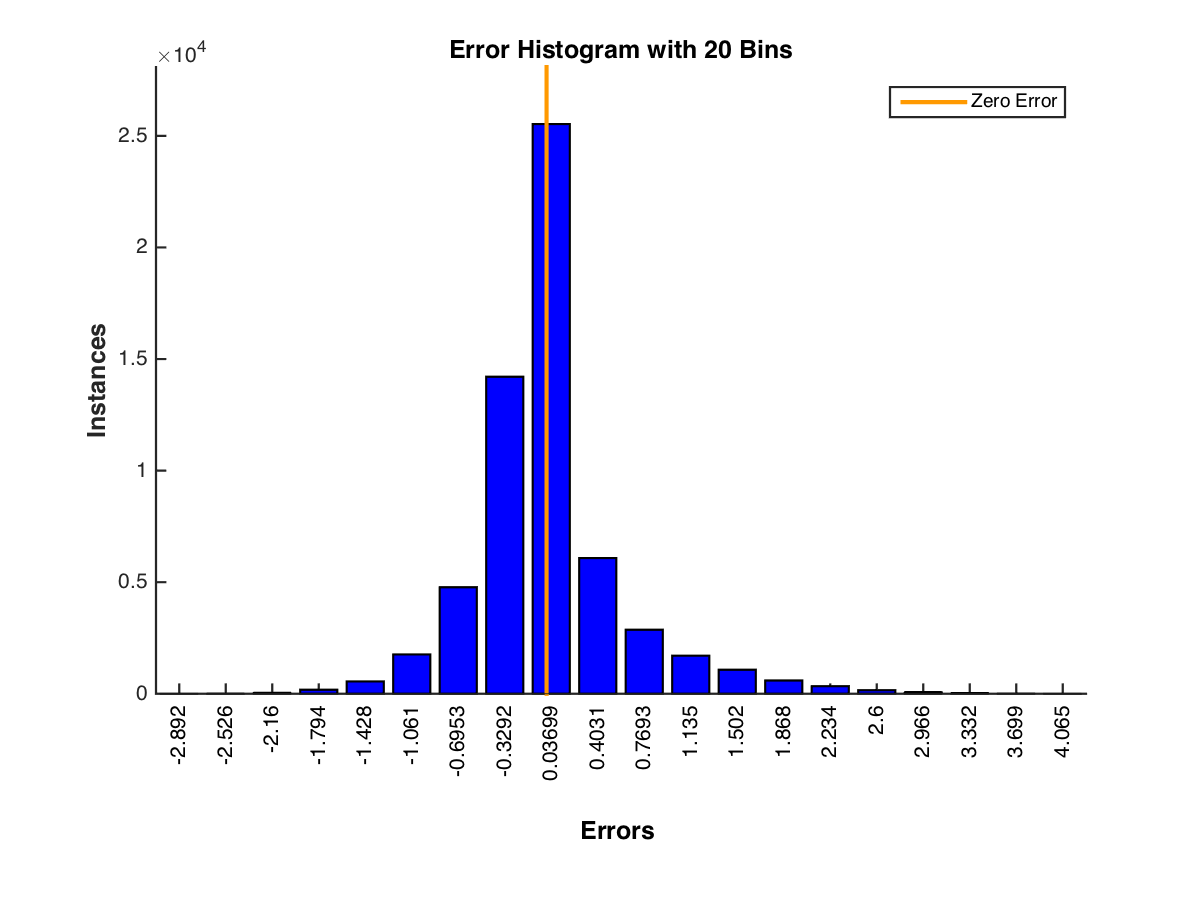
\includegraphics[scale=0.28]{ploterrhist_20.png}
}
\subfigure[Train-Validation-Test error plot for 50 neuron hidden layer]{
    \label{fig:nn-runs50}
    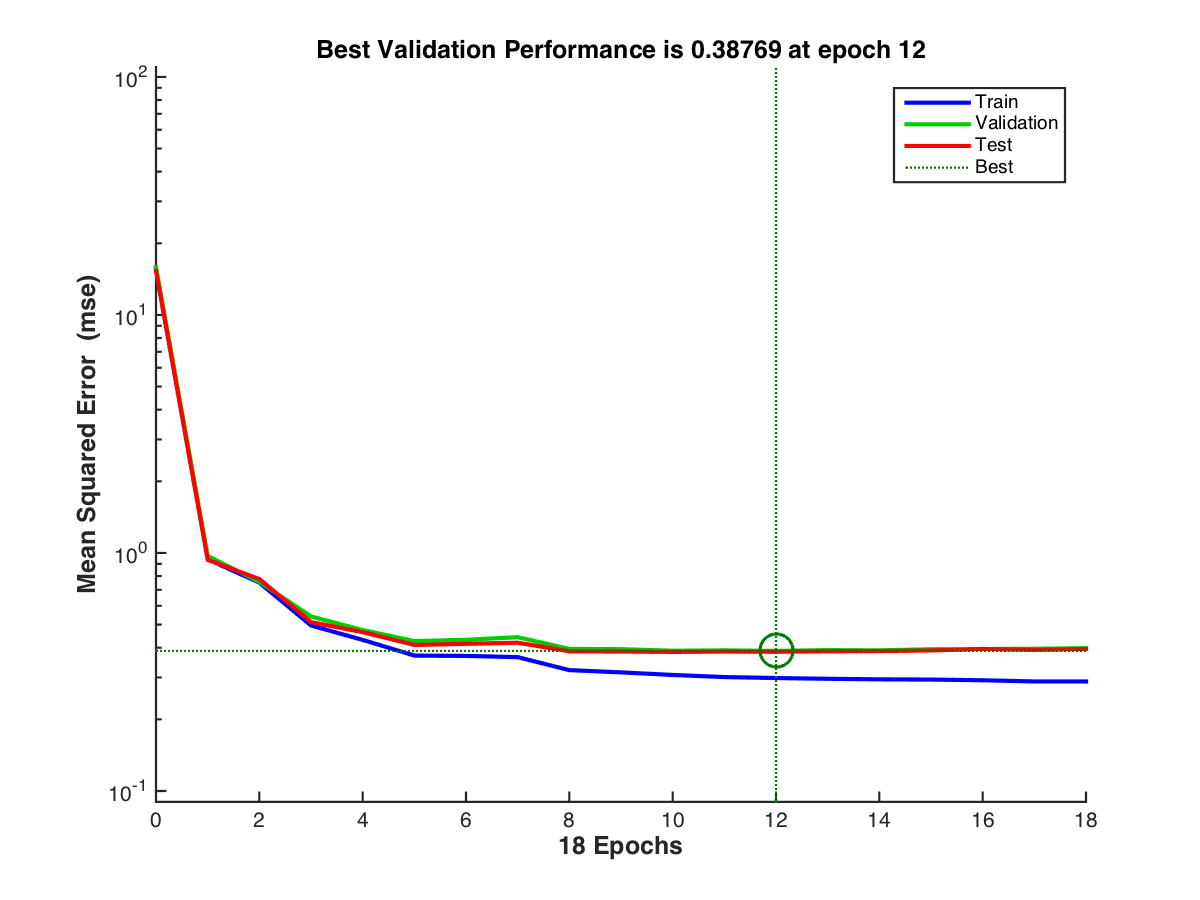
\includegraphics[scale=0.28]{plotperform_50.png}
}
\subfigure[Error distribution histogram for 50 neuron hidden layer]{
    \label{fig:nn-runs}
    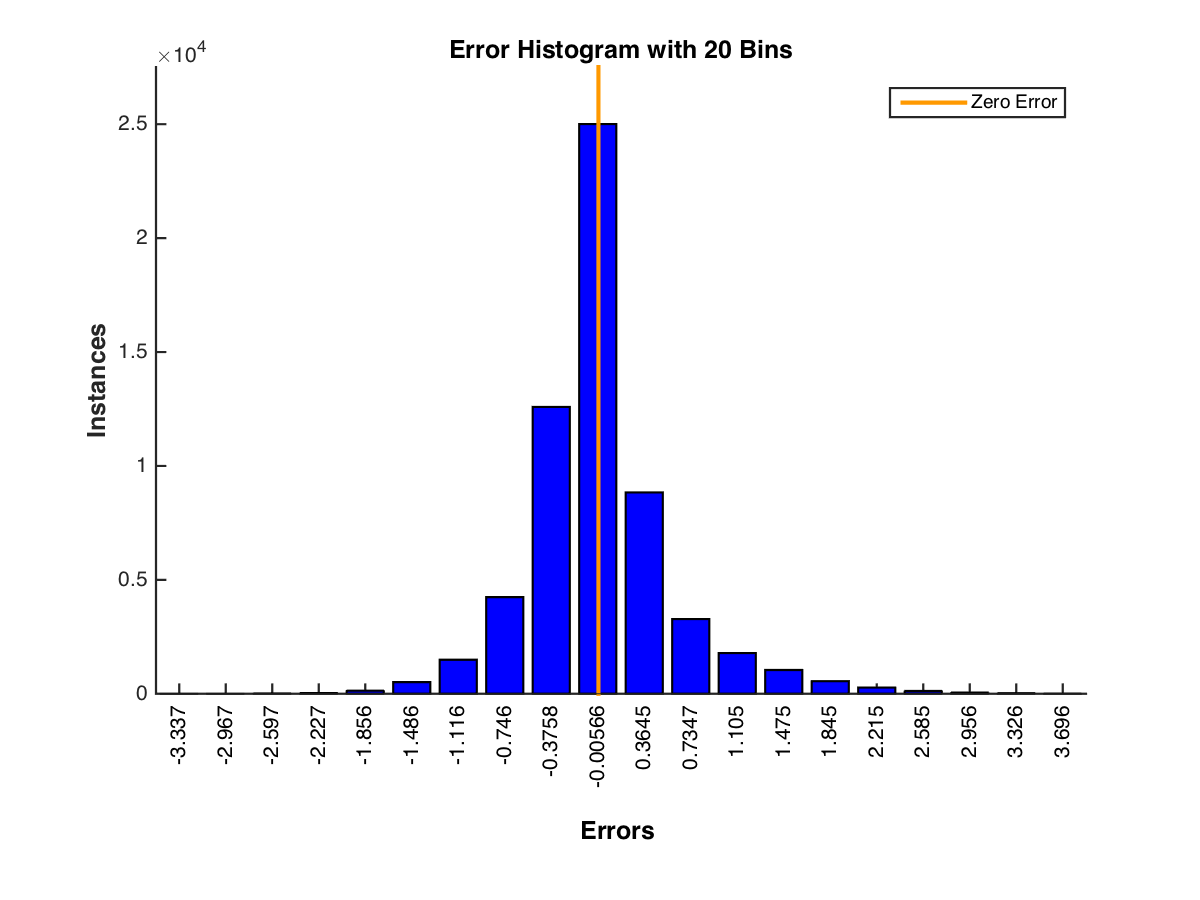
\includegraphics[scale=0.28]{ploterrhist_50.png}
}
\caption[]{Plots of various Train-Validation-Test error for number of neurons = [10, 20, 50]}
\label{fig:nn-runs}
\end{figure}

\subsubsection*{Deep Networks}
For this project, we tried using deep networks as well. The deep network was made using PyBrain. We tried using different activation functions and architectures to understand how deep networks would work. The architecture shown in \autoref{fig:nn_deep} had 3 layers - visible later contains 91 neurons, the first hidden layer (\texttt{tanh}) had 91 neurons, the second hidden layer (\texttt{sigmoid}) had 50 neurons, the third hidden layer (\texttt{sigmoid}) had 20 neurons, and the output layer had 1 linear node.

\begin{center}
\begin{neuralnetwork}[height=7]
		\newcommand{\nodetextclear}[2]{}
		\newcommand{\nodetexty}[2]{$y_#2$}
		\inputlayer[count=4, bias=true, title=Input\\layer]
		\hiddenlayer[count=7, bias=true, title=Hidden layer (Hyperbolic Tangent Layer), text=\nodetextclear] \linklayers
		\hiddenlayer[count=6, bias=true, title=Hidden layer (Sigmoid Layer), text=\nodetextclear] \linklayers
		\hiddenlayer[count=5, bias=true, title=Hidden layer(Sigmoid Layer), text=\nodetextclear] \linklayers
		\outputlayer[count=1, title=Output\\layer, text=\nodetexty] \linklayers
\label{fig:nn_deep}
\end{neuralnetwork}
\end{center}

\subsection{Gradient Boosting}
\subsection{Random Forests}
\section{Ensemble of all Learners}

\section{Conclusion}
\label{sec:conclusion}

\begin{thebibliography}{}
\end{thebibliography}
\end{document}

